\paragraph{}{
	Le second circuit électronique composant le processeur est
	le contrôleur de sauts. Son rôle est de mettre à jour le pointeur
	d'instructions \textit{PC} (pour \textit{Program Counter})
	en fonction du résultat de l'opération que vient d'effectuer
	l'UAL pour le cycle suivant. Le saut est déterminé en fonction
	des indicateurs que le circuit a en entrée. C'est-à-dire 
	\textit{SF} et \textit{ZF}. Pour ce là, on fait une table de
	vérité présente à la figure \ref{ctrl_saut_tv}. Une 
	fois la	table remplie, on en tire l'équation suivante :
	\begin{equation}
		\label{ctrl_saut_eq}
		\begin{split}
		C_{1} = & \neg C_{1} . O_{1} . \neg O_{0} . \neg{ZF} \\
				& + \neg O_{2} . O_{1} . O_{0} .  {ZF} \\
				& + O_{2} . \neg O_{1} . O_{0} . \neg{ZF} . {SF} \\
				& + O_{2} . O_{1} . \neg{ZF} . \neg{SF} \\
				& + O_{2} . O_{1} . O_{0} . ( {ZF} + \neg{ZF} . {SF}) \\
				& + O_{2} . O_{1} . O_{0} . ( {ZF} + \neg{ZF} . \neg{SF} ) \\
		\end{split}
	\end{equation}
	On traduit alors l'équation en circuit et on obtient le circuit
	de la figure \ref{control_saut_circ}.
}

\paragraph{}{
	Dans l'équation \ref{ctrl_saut_eq}, $O_{i}$ correspond au $i$-ème
	bit de l'opcode. La variable $C_{1}$ nous renseigne lorsqu'il faut faire un saut.
	Enfin, \textit{ZF} et \textit{SF} correspondent aux drapeaux levés par l'UAL.
}

\begin{figure}[!ht]
	\centering
	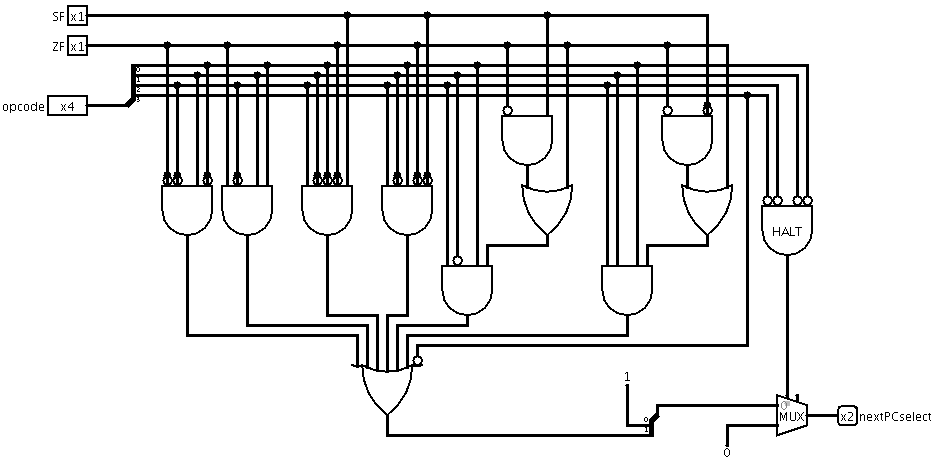
\includegraphics[scale=0.4,origin=c]{circuits/control_saut.png}
	\caption{\label{control_saut_circ} Sch\'{e}ma \'{e}lectronique du contr\^{o}leur de sauts}
\end{figure}

\paragraph{}{
	Le multiplexeur qui contrôle \textit{PC} réponds au codage suivant:
	À la fin du programme, pour l'instruction \textit{halt}, le code du
	multiplexeur est $00$, pour aller à la prochaine instruction on envoie
	$11$. Enfin, lors d'un saut on y envoie $01$.
}

\begin{figure}
	\centering
	\begin{tabular}{|c|c|c|c|c|c|}
		\hline 
		$O_{2}$ & $O_{1}$ & $O_{0}$ & ZF & SF & $C_{1}$ \\ 
		\hline 
		$0$ & $0$ & $1$ & $\times$ & $\times$ & $0$ \\ 
		\hline 
		$0$ & $1$ & $0$ & $0$ & $\times$ & $1$ \\ 
		\hline 
		$0$ & $1$ & $0$ & $0$ & $\times$ & $0$ \\ 
		\hline 
		$0$ & $1$ & $1$ & $1$ & $\times$ & $0$ \\ 
		\hline 
		$0$ & $1$ & $1$ & $1$ & $\times$ & $1$ \\ 
		\hline 
		$1$ & $0$ & $0$ & $0$ & $0$ & $0$ \\ 
		\hline 
		$1$ & $0$ & $0$ & $0$ & $1$ & $1$ \\ 
		\hline 
		$1$ & $0$ & $0$ & $1$ & $0$ & $0$ \\ 
		\hline 
		$1$ & $0$ & $0$ & $1$ & $1$ & $0$ \\ 
		\hline 
		$1$ & $0$ & $1$ & $0$ & $0$ & $1$ \\ 
		\hline 
		$1$ & $0$ & $1$ & $0$ & $1$ & $0$ \\ 
		\hline 
		$1$ & $0$ & $1$ & $1$ & $0$ & $0$ \\ 
		\hline 
		$1$ & $0$ & $1$ & $1$ & $1$ & $0$ \\ 
		\hline 
		$1$ & $1$ & $0$ & $0$ & $0$ & $0$ \\ 
		\hline 
		$1$ & $1$ & $0$ & $0$ & $1$ & $1$ \\ 
		\hline 
		$1$ & $1$ & $0$ & $1$ & $0$ & $1$ \\ 
		\hline 
		$1$ & $1$ & $0$ & $1$ & $1$ & $1$ \\ 
		\hline 
		$1$ & $1$ & $1$ & $0$ & $0$ & $1$ \\ 
		\hline 
		$1$ & $1$ & $1$ & $0$ & $1$ & $0$ \\ 
		\hline 
		$1$ & $1$ & $1$ & $1$ & $0$ & $1$ \\ 
		\hline 
		$1$ & $1$ & $1$ & $1$ & $1$ & $1$ \\ 
		\hline 
	\end{tabular} 
	\caption{\label{ctrl_saut_tv} Table de vérité du contrôleur de sauts}
\end{figure}

\paragraph{}{
	Penchons-nous maintenant sur le décodeur d'instructions.
}